\documentclass[12pt, AutoFakeBold=4]{ctexart}

\setmainfont{Times New Roman}
\setCJKmainfont{SimSun}

\usepackage{tikz, amsmath, graphics, graphicx,listings, amsmath}

\usepackage[hyperref, UTF8]{ctex}
\usepackage[pagebackref]{hyperref}

\usetikzlibrary{shapes, arrows, positioning, calc}
\usepackage{caption, xcolor, times, enumitem, fontspec}

\usepackage[table]{xcolor}
\usepackage{booktabs,tabularx,makecell,multirow,float}
\usepackage{standalone}

\usepackage[a4paper]{geometry}
\usepackage{gbt7714}
\usepackage{sim-os-menus}
\usepackage{minted}

\usepackage{animate}
\usepackage{algorithm}
\usepackage{algorithmic}

\usetikzlibrary{patterns}
\counterwithin{figure}{subsection}
\counterwithin{table}{subsection}
\counterwithin{listing}{subsection}


% Codes Block
\setmonofont{Consolas}   % 设置等宽字体
\lstset{
	language=Python, % 设置语言为 Python
	basicstyle=\ttfamily\small, % 设置代码字体和大小
	numbers=none, % 显示行号
	numberstyle=\tiny, % 行号字体
	stepnumber=1, % 每行显示行号
	frame=none, % 给代码加框
	captionpos=b, % bottom
	breaklines=true, % 自动换行
	keywordstyle=\color{blue}, % 关键字颜色
	commentstyle=\color{green!50!black}, % 注释颜色
	stringstyle=\color{red}, % 字符串颜色
	showstringspaces=false % 不显示字符串中的空格
}

\setminted{
	fontsize=\small,    % 设置字体大小
	breaklines,         % 自动换行
	framesep=2mm,       % 边框与代码的间距
}

\hypersetup{
	colorlinks = true,
	linkcolor = blue!80!black,
	citecolor = green!60!black,
	urlcolor  = pink!70!black,
	pdftitle = {增强型目录示例},
	bookmarksdepth = 3
}


\definecolor{headbg}{RGB}{63,81,181}   % 表头蓝
\definecolor{rowhi}{RGB}{245,245,245}  % 行高亮
\definecolor{pros}{RGB}{232,245,233}   % 优点底色
\definecolor{cons}{RGB}{255,235,238}   % 缺点底色
\colorlet{myred}{red!80!black}
\colorlet{myblue}{blue!80!black}
\colorlet{mygreen}{green!60!black}
\colorlet{myorange}{orange!70!red!60!black}
\colorlet{mydarkred}{red!30!black}
\colorlet{mydarkblue}{blue!40!black}
\colorlet{mydarkgreen}{green!30!black}

% Icon Setting
\usepackage{fontawesome5}
\usepackage{forest}
\newcommand{\texicon}{{\color{blue}\faFileCode}}
\newcommand{\pdficon}{\color{red}\faFilePdf}
\newcommand{\pyicon}{\color{green}\faPython}
\newcommand{\mdicon}{\color{blue!50!black}\faMarkdown}

\title{\zihao{3}\heiti 基于神经网络的系统辨识}
\date{}


\begin{document}
	\thispagestyle{empty}
	
	\begin{tikzpicture}[remember picture, overlay]
		\draw[dashed] ($(current page.north)+(-9cm,0)$)--($(current page.south)+(-9cm,0)$);
		\fill[black] (-2.55,-1) rectangle(-2.4,-2.8);
		\fill[black] (-2.55,-14) rectangle(-2.4,-15.8);
		
		\node[draw=black,fill=white,line width=1pt,minimum width=1.5cm,minimum height=1.5cm,anchor=north east] at ($(current page.north east)+(-3cm,-2cm)$) (rect1) {成绩};
		
		\node[draw=black,fill=white,line width=1pt,minimum width=1.5cm,minimum height=1.5cm,anchor=north east] at ($(current page.north east)+(-1.5cm,-2cm)$) (rect2) {};
		
	\end{tikzpicture}
	
	
	\begin{center}
		
		\begin{figure}[t]
			\centering
			\includegraphics[width=0.4\textwidth]{E:/texlive/Tex_path/texstudio/TexTablet/texstudio/JIT.font.jpg}
		\end{figure}
		\vspace{0.1cm}
		
		{
			\zihao{0}\CJKfontspec{华文行楷.ttf}\textbf{{人 工 智 能 大 作 业}}\par
		\LARGE\textbf{ (理工类)}
		}		
		\begin{figure}[htpb]
			\centering
			\includegraphics[width=0.22\textwidth]{E:/texlive/Tex_path/texstudio/TexTablet/texstudio/JIT.flag.bw.png}
		\end{figure}
		\par
		\vspace{4cm}
		
		{\zihao{4}\heiti 
			\makebox[1.8cm][c]{课程名称:}\underline{\makebox[5cm][c]{人工智能}}\hspace{0.4cm}
			\makebox[1.8cm][c]{专业班级:}\underline{\makebox[5.5cm][c]{24自动化(W专转本)}}\\
			\vspace{0.6cm}
			
			\makebox[1.8cm][c]{学生学号:}\underline{\makebox[5cm][c]{2417504036}}\hspace{0.55cm}
			\makebox[1.8cm][c]{学生姓名:}\underline{\makebox[5.4cm][c]{陈亚鹏}}\\
			\vspace{0.6cm}
			
			\makebox[1.8cm][c]{所属院部:}\underline{\makebox[5.2cm][c]{\zihao{-4}智能科学与控制工程学院}}\hspace{0.4cm}
			\makebox[1.8cm][c]{指导老师:}\underline{\makebox[5.2cm][c]{张\ 艳}}\\
		}
		\vspace{1cm}
		
		{\zihao{3}\heiti
			20\underline{\makebox[0.8cm]{ 24 }}——20\underline{\makebox[0.8cm]{ 25 }}学年 \hspace{1.8cm} 第\underline{\makebox[0.8cm]{ 二 }}学期\\
			\vspace{1cm}
		
		金陵科技学院教务处制
	}
	\end{center}
	\newpage
	
	%***************************************************************************%
	\thispagestyle{empty}
	\maketitle
	\tableofcontents
	\newpage
	\pagenumbering{arabic}
	%****************************************************************************%
	\section{绪论}
	\subsection{研究背景与意义}
随着人工智能技术的快速发展,神经网络在系统辨识中的应用得到了广泛关注。系统辨识是通过实验数据建立动态系统数学模型的过程,在控制工程、机器人学和工业自动化等领域具有重要意义。\cite{ai_book1}
然而,传统的系统辨识方法在处理复杂非线性系统时存在局限性,而神经网络凭借其强大的非线性拟合能力,为系统辨识提供了一种高效的解决方案。
神经网络的系统辨识方法可以通过输入-输出数据直接拟合系统的动态特性,避免了复杂的物理建模过程。这种方法不仅提高了辨识精度,还显著降低了计算成本,为复杂系统的建模和控制提供了新的思路。

\subsection{本文研究内容的安排}
本文主要研究基于神经网络的一阶倒立摆系统辨识方法,并结合 PID 控制器对系统进行校正。全文内容安排如下:
\begin{enumerate}
    \item 第一节绪论:介绍研究背景与意义,并说明本文的研究内容。
    \item 第二节算法原理介绍:阐述倒立摆的动力学演化过程,以及神经网络在系统辨识中的工作原理,并绘制多层感知机(MLP)的结构图和流程图。
    \item 第三节程序与运行结果:基于倒立摆模型进行系统辨识,给出程序代码和仿真结果,并结合 PID 控制器对系统进行校正。
    \item 第四节总结:总结本文的研究内容和成果,并展望未来的研究方向。
\end{enumerate}

\newpage

	\section{算法原理介绍}
		\subsection{一阶倒立摆的动力学方程}
	倒立摆是一个典型的非线性、不稳定系统。目标是通过控制输入(如力矩或推力)使摆杆保持在直立平衡位置(目标角度为 0 弧度)。
	\input{pendulum_fig.tex}
	写下动力学方程:
	\begin{equation}
		\frac{\mathrm{d^2\theta}}{\mathrm{dt^2}}+\frac{b}{m}\frac{\mathrm{d\theta}}{\mathrm{dt}}-\frac{g}{l}\mathrm{\sin(\theta)}=\frac{\tau}{m l^2}
	\end{equation}
	\par
	
	相空间方程:
	\begin{equation}
		\left\{
		\begin{array}{c}
			\dot{\theta}=\omega\\
			\dot{\omega}= g/l \ \mathrm{\sin(\theta)}
			-b/m\ \omega + \tau/(m l^2)
		\end{array}
		\right.
	\end{equation}
	
	其中:
	\begin{itemize}
		\item \(\theta\):摆角(角度)。
		\item \(\dot{\theta}\):角速度。
		\item \(\ddot{\theta}\):角加速度。
		\item \(g\):重力加速度。
		\item \(l\):摆长。
		\item \(b\):阻尼系数。
		\item \(m\):摆的质量。
		\item \(\tau\):控制力矩。
	\end{itemize}
	
	
	\subsection{神经网络的工作原理}
神经网络是一种模拟生物神经系统的计算模型,具有强大的非线性拟合能力。多层感知机(MLP)是神经网络的基本结构,由输入层、隐藏层和输出层组成\cite{ai_book2}。通过数据训练神经网络,进行非线性系统辨识通过拟合系统的输入与输出之间的非线性映射关系,从而建立一个能够近似描述系统动态行为的模型,从而实现系统辨识。

\subsection{MLP 结构图}
以下是 MLP 结构图以及权重、阈值更新公式:\par
\begin{figure}[H]
	\centering
	\includegraphics{MLP.pdf}
\end{figure}
	


\subsection{系统辨识流程图}
以下是基于神经网络的系统辨识流程图:
\begin{figure}[H]
    \centering
    \begin{tikzpicture}[node distance=2cm]
        \node[rectangle, draw, fill=blue!20, text width=4cm, align=center] (start) {输入-输出数据};
        \node[rectangle, draw, fill=green!20, text width=4cm, align=center, below of=start] (train) {训练神经网络};
        \node[rectangle, draw, fill=red!20, text width=4cm, align=center, below of=train] (model) {得到系统模型};
        \node[rectangle, draw, fill=yellow!20, text width=4cm, align=center, below of=model] (predict) {预测系统输出};

        \draw[->] (start) -- (train);
        \draw[->] (train) -- (model);
        \draw[->] (model) -- (predict);
    \end{tikzpicture}
    \caption{基于神经网络的系统辨识流程图}
\end{figure}\par
{\Large \heiti 详细步骤}
\begin{enumerate}
\item {\heiti 数据采集}
收集系统的输入 ( u(t) ) 和输出 ( y(t) ) 数据,形成数据集:$  \mathcal{D} = {(u(t), y(t)) \mid t = 1, 2, \dots, N} $

\item {\heiti 数据预处理}
对数据进行归一化或标准化处理:$  u'(t) = \frac{u(t) - \mu_u}{\sigma_u}, \quad y'(t) = \frac{y(t) - \mu_y}{\sigma_y} $

\item {\heiti 神经网络建模}
选择神经网络结构(如前馈网络、递归网络)并定义模型: $ \hat{y}(t) = f_\theta(u(t), y(t-1), y(t-2), \dots)  $
\item {\heiti 损失函数定义}
定义损失函数(如均方误差)以衡量预测值与真实值的差异: $ \mathcal{L}(\theta) = \frac{1}{N} \sum_{t=1}^N \left( y(t) - \hat{y}(t) \right)^2 $

\item {\heiti 模型训练}
使用优化算法(如梯度下降、Adam)最小化损失函数:$  \theta^* = \arg\min_\theta \mathcal{L}(\theta) $

\item {\heiti 模型验证}
在验证集上评估模型性能,计算误差指标(如均方误差、平均绝对误差):$  \text{MSE} = \frac{1}{M} \sum_{t=1}^M \left( y_{\text{true}}(t) - \hat{y}(t) \right)^2 $

\item {\heiti 模型部署}
将训练好的模型用于实时预测或控制:$  \hat{y}(t) = f_{\theta^*}(u(t), y(t-1), y(t-2), \dots) $
\end{enumerate}
\newpage

	\section{程序与运行结果}

	\subsection{系统辨识程序}
	\label{subsect:3.1}
	开始训练一个神经网络,这里仅展示核心代码(示例程序):
	\begin{itemize}
\item 定义动力学方程模型,生成数据集:
\begin{PYViewer}[width=15cm]{}
	\begin{minted}{python}
# 倒立摆动力学方程
def inverted_pendulum(state, t, g, l, b, m, tau):
theta, omega = state
dtheta_dt = omega
domega_dt = (g / l) * np.sin(theta) - (b / m) * omega\
 + tau / (m * l**2)
return [dtheta_dt, domega_dt]

# 数据生成
def generate_data():
    g, l, b, m = 9.8, 1.0, 0.1, 1.0  # 参数
    t = np.linspace(0, 10, 1000)  # 时间
    tau = 0  # 控制力矩
    y0 = [0.1, 0.0]  # 初始条件 [初始角度, 初始角速度]
    data = odeint(inverted_pendulum, y0, t,\
     args=(g, l, b, m, tau))
    theta, omega = data[:, 0], data[:, 1]
    dtheta_dt = omega
    domega_dt = (g / l) * np.sin(theta) - (b / m) * omega\
    + tau / (m * l**2)
    X = np.column_stack((theta, omega,\
     tau * np.ones_like(theta)))  # 输入 [角度, 角速度, 控制力矩]
    y = domega_dt  # 输出 [角加速度]
    return X, y, t, data
\end{minted}
\end{PYViewer}


\item 训练神经网络
\begin{PYViewer}[width=15cm]{}
	\begin{minted}{python}
# 生成数据
X, y, t, data = generate_data()

# 划分训练集和测试集
X_train, X_test, y_train, y_test = \
train_test_split(X, y, test_size=0.2, random_state=42)

# 神经网络建模
model = MLPRegressor(hidden_layer_sizes=(128, 128),\
activation='relu', max_iter=5000, random_state=42)
model.fit(X_train, y_train)

# 预测
y_pred = model.predict(X_test)

# 评估
mse = mean_squared_error(y_test, y_pred)
print(f"Mean Squared Error: {mse}")
	\end{minted}
\end{PYViewer}

\noindent\hfil\fbox{\parbox{0.8\textwidth}{\centering
		\color{blue}Mean Squared Error: 0.009241777330554795}}\hfil\par
这里的示例程序设置了两层隐藏层,每层神经元大小为128,使用Relu作为激活函数,训练轮数为5000轮。神经网络接受的输入参数有当前摆的角度$\theta$,角加速度$\omega$以及控制力矩$\tau$, 输出为角加速度$\dot{\omega}$。 
	\end{itemize}


\subsection{仿真结果}
通过神经网络给出的预测角加速度结合Euler法可以给出预测的动力学演化过程,见图\ref{图:动力学}.
这里设置初始角度$\theta_0=0.1 rad$,初始角速度$\omega_0=0.0rad/s$,控制力矩$\tau=0N\cdot m$。\colorbox{blue}{—}为数值解,\colorbox{red}{--}为MLP的预测值。
\begin{figure}[htpb]
    \centering
    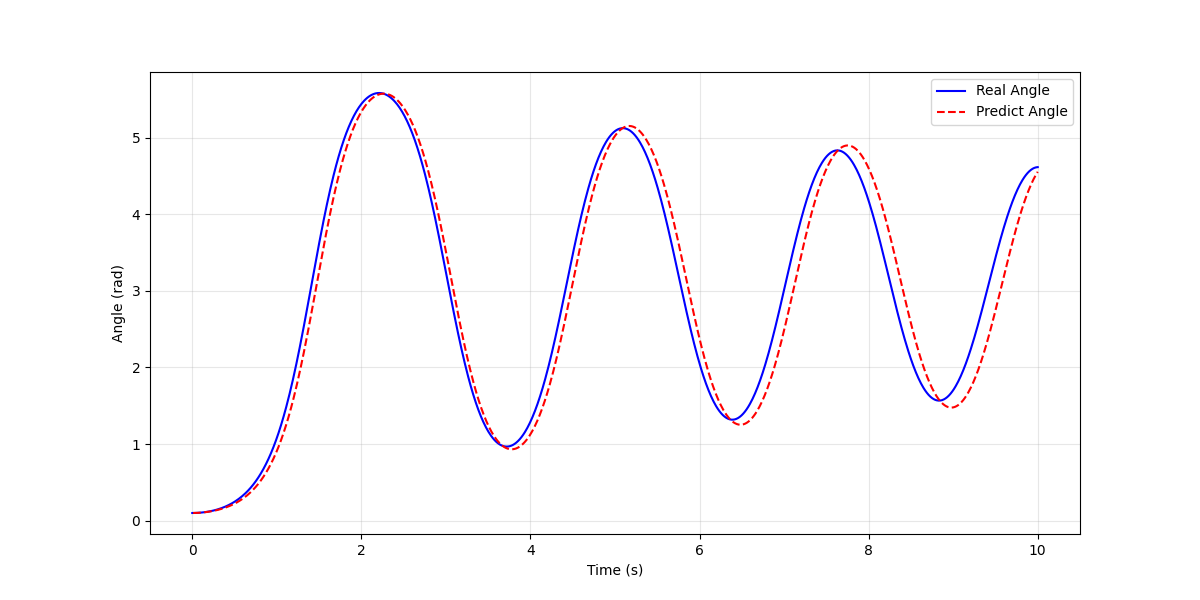
\includegraphics[width=0.8\textwidth]{evolutionary.png}
    \caption{齐次方程的动力学过程}
    \label{图:动力学}
\end{figure}
\par
初始角度$\theta_0=0.0 rad$,初始角速度$\omega_0=0.0rad/s$,控制力矩$\tau=1N\cdot m$。
\begin{figure}[htpb]
	\centering
	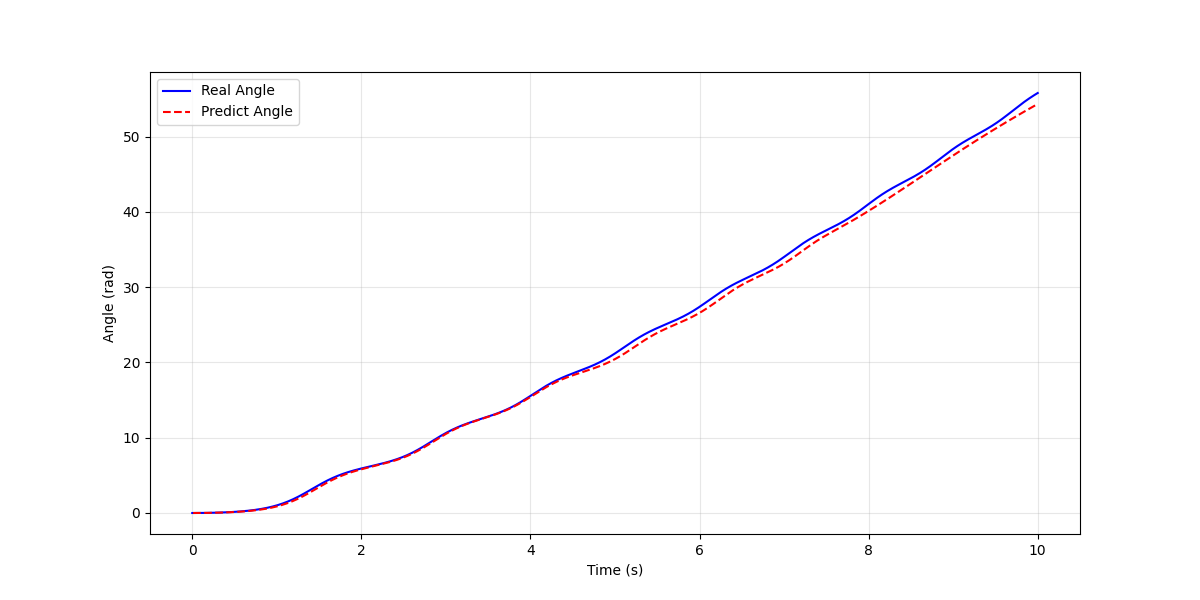
\includegraphics[width=0.8\textwidth]{evolut.png}
	\caption{非齐次方程的动力学过程}
	\label{图:动力学2}
\end{figure}

\subsection{PID 校正}
若使用\ref{subsect:3.1}的示例程序所训练出来的神经网络并不是普遍cover的。换句话说,这个模型的泛化能力不是很好。如果要改善性能需要加不同初始条件下以及不同控制力矩的数据集。下面将采用我已经训练好的一套神经网络来进行PID校正。注意,图\ref{图:PID}是在神经网络上得到的结果。在进行完PID校正后,我们仍需要仿真/物理实验去验证模型和参数的有效性。
\begin{algorithm}
	\caption{PID 控制器伪码}
	\begin{algorithmic}[1]
		\REQUIRE $K_p$, $K_i$, $K_d$ (PID 增益参数)
		\REQUIRE $setpoint$ (目标值), $current$ (当前值), $dt$ (时间步长)
		\STATE $prev\_error \gets 0$ \COMMENT{初始化前一时刻误差}
		\STATE $integral \gets 0$ \COMMENT{初始化积分项}
		
		\WHILE{系统运行中}
		\STATE $error \gets setpoint - current$ \COMMENT{计算当前误差}
		\STATE $integral \gets integral + error \cdot dt$ \COMMENT{更新积分项}
		\STATE $derivative \gets (error - prev\_error) / dt$ \COMMENT{计算误差的变化率}
		\STATE $output \gets K_p \cdot error + K_i \cdot integral + K_d \cdot derivative$ \COMMENT{计算控制输出}
		\STATE $prev\_error \gets error$ \COMMENT{更新前一时刻误差}
		\STATE 应用 $output$ 到系统
		\ENDWHILE
	\end{algorithmic}
\end{algorithm}
\begin{figure}[htpb]
	\centering
	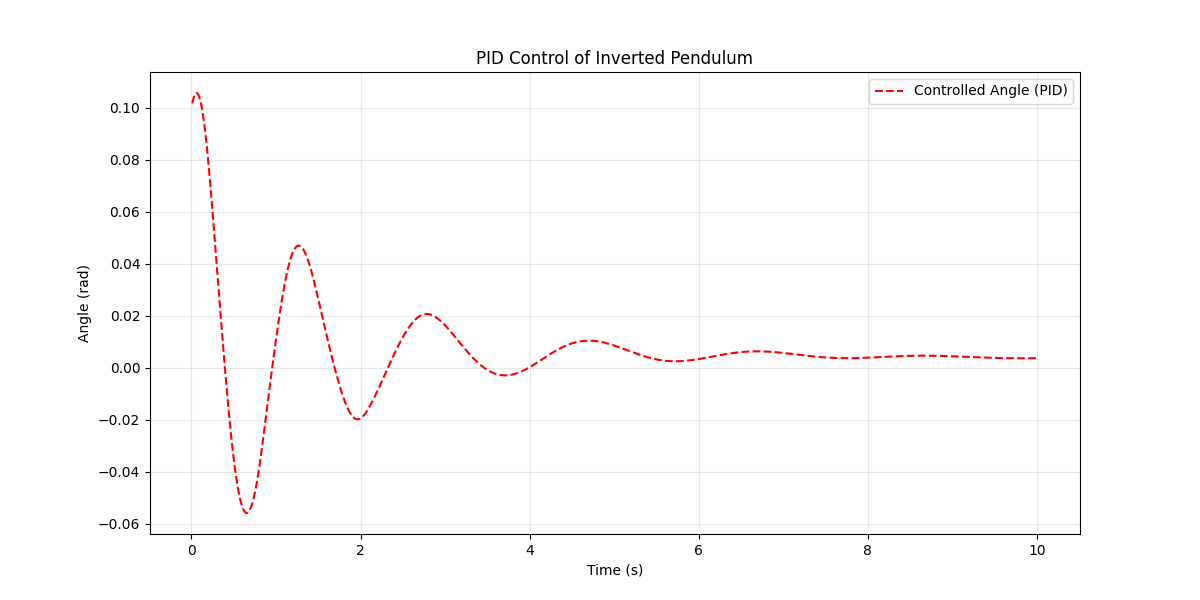
\includegraphics[width=0.85\textwidth]{PID.png}
	\caption{未优化前参数给出的PID校正}
	\label{图:PID}
\end{figure}

PID 控制器通过实时调整控制力矩,校正倒立摆的偏差,使其保持直立稳定。比例控制提供快速响应,积分控制消除稳态误差,微分控制抑制振荡。
 对于参数$k_P,k_I,k_D$的确定有多种方法,图\ref{图:PID}是基于图\ref{图:动力学}做的PID校正,设置的参数为$k_P=50,k_I=2,k_D=2$.当然不是最优的,甚至不是局部最优的。现使用GA算法进行参数的优化,以下展示了在终端上运行GA算法的迭代过程。\par
 
\begin{TermWin}[width=15cm]{}
Generation 1: Best Fitness = 44.26614012560816, Best PID = [13.38137479  9.9421895   5.99600607]
...
Generation 30: Best Fitness = 7.4091762529322365, Best PID = [36.97944279  3.61454539  8.16905168]
...
Generation 36: Best Fitness = 6.984666953068312, Best PID = [42.44913587  3.85688028  7.83797342]
...
Optimal PID Parameters: Kp = 52.07405094371485, Ki = 6.0892017239746385, Kd = 9.146399457554605
\end{TermWin}
选定PID参数为$k_P=52.074,k_I=6.0893,k_D=9.1464$.
\begin{figure}[htpb]
	\centering
	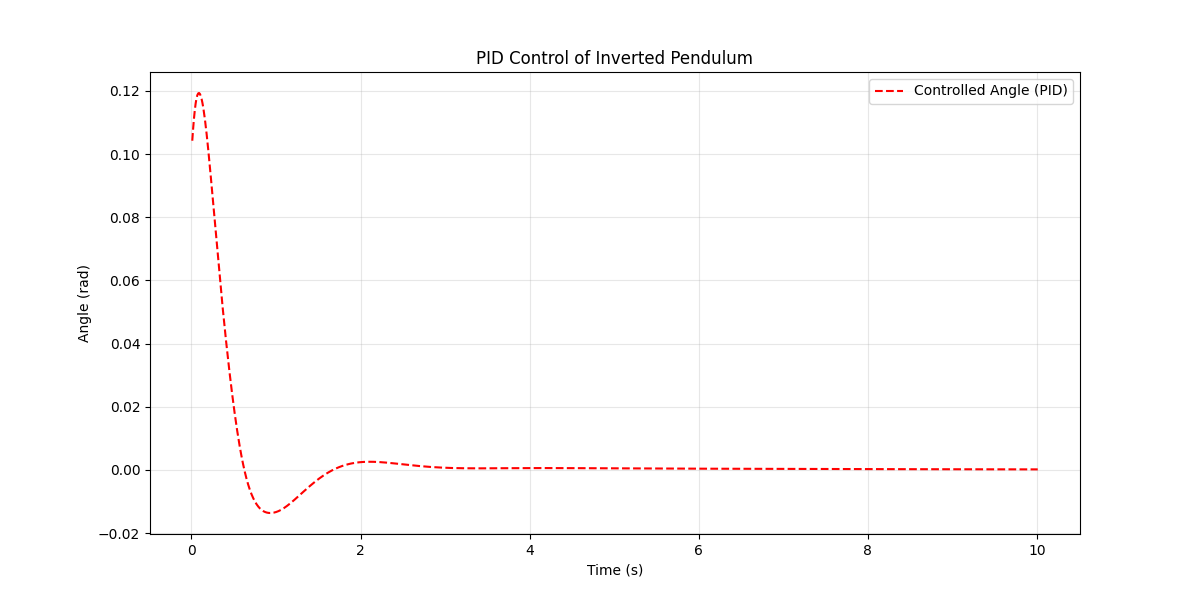
\includegraphics[width=0.85\textwidth]{PID-Best.png}
	\caption{GA算法给出的PID参数校正}
	\label{图:PID-Best}
\end{figure}
\par
这里的图\ref{图:PID-Best}也是初始角度为0.1 rad的PID控制。显然控制效果优于图\ref{图:PID}的结果。\par
现考虑将这套PID参数应用到真实倒立摆系统上,并分析控制效果。\par
\begin{figure}[htpb]
	\centering
	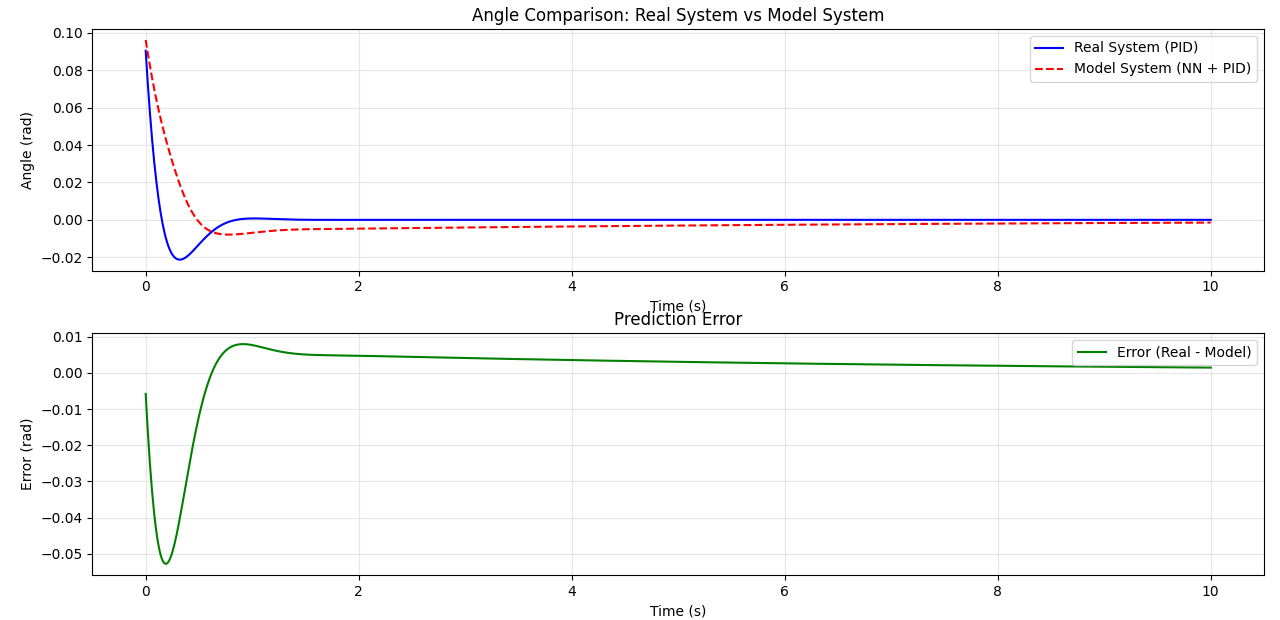
\includegraphics[width=\textwidth]{Real-Model.png}
	\caption{比较及模型误差}
	\label{图:Real-Model}
\end{figure}
使用平均绝对误差作为评价函数:
$$
\text{MAE} = \frac{1}{n} \sum_{i=1}^{n} |y_{\text{real}, i} - y_{\text{model}, i}| 
$$
\noindent\hfil\fbox{\parbox{\textwidth}{\centering
		\color{blue}Mean Absolute Error (MAE): 0.0049}}\hfil\par
	
从图\ref{图:Real-Model}中会发现一个很有意思的事情,实际模型给出的预测值和真实值之间还是有着些许差异的。如果要求训练出更接近真实系统的神经网络模型,可以通过以下几点实现(不限于):
\begin{itemize}
	\item 增加训练数据的多样性
	\item 增加训练数据的分辨率
	\item 增加隐藏层或神经元数量
\end{itemize}

\newpage

	\section{总结}
	本文研究了基于神经网络的一阶倒立摆系统辨识方法,并结合 PID 控制器对系统进行了校正。通过仿真实验验证了神经网络在系统辨识中的有效性,以及 PID 控制器在系统校正中的作用。未来可以进一步研究更复杂的非线性系统辨识方法,并结合强化学习优化控制策略。\par
	整个项目已开源到个人\href{https://github.com/YapengChen1102/AI-Homework}{\color{magenta}{GitHub}}上。核心文件的作用如下:\par

	\begin{ForestDirTree}%
		[font=\sffamily,coliconfolder=yellow!50!pink,iconfiles,coliconfile=teal,vsep=0.5em]%
		{}
		[AI-Homework,FTdir
			[\texicon\ 36-AI.tex\hspace{6cm}	\LaTeX 文件]
			[\pdficon\ 36-AI.pdf\hspace{6cm}	{\normalcolor 我的大作业(本文档)}]
			[\pyicon\ MLP-Design.py\hspace{4.8cm}	{\normalcolor 训练神经网络的程序}]
			[\pyicon\ test.py\hspace{6.4cm}	{\normalcolor 用于测试比较}]
			[\pyicon\ GA.py\hspace{6.4cm}	{\normalcolor 遗传算法的程序}]
			[\pyicon\ Demo.py\hspace{6cm}	{\normalcolor 添加PID控制的程序}]
			[\pyicon\ simulation\_animation.py\hspace{3cm}	{\normalcolor 倒立摆的仿真程序}]
			[mlp\_model.joblib\hspace{4.5cm} {\normalcolor 神经网络模型(必要)} ,FTfile]
			[\mdicon\ README.md]
		]
	\end{ForestDirTree}
	
	\addcontentsline{toc}{section}{参考文献}
	\bibliographystyle{gbt7714-author-year}
	\bibliography{refer.bib}
\end{document}
